\chapter{Конструкторский раздел}
В конструкторском разделе спроектировано разрабатываемое программное обеспечение и формально описаны используемые алгоритмы.

\section{Функциональная диаграмма}
На рисунке~\ref{fig:a0} представлена IDEF0-диаграмма визуализации сцены уровня A0.
\begin{figure}[ht!]
	\centering
	\includesvg[width=0.7\textwidth]{cloud_a0.svg}   
	\caption{IDEF0-диаграмма функциональной декомпозиции уровня A0}
	\label{fig:a0}
\end{figure}

На рисунке~\ref{fig:a1} представлена IDEF0-диаграмма визуализации сцены уровня A1.
\begin{figure}[ht!]
	\centering
	\includesvg[width=1.0\textwidth]{cloud_a1.svg}   
	\caption{IDEF0-диаграмма функциональной декомпозиции уровня A1}
	\label{fig:a1}
\end{figure}
\clearpage

\section{Схемы алгоритмов}

На рисунке~\ref{fig:cloud_fc} представлена схема алгоритма отрисовки облака.
\begin{figure}[ht!]
	\centering
	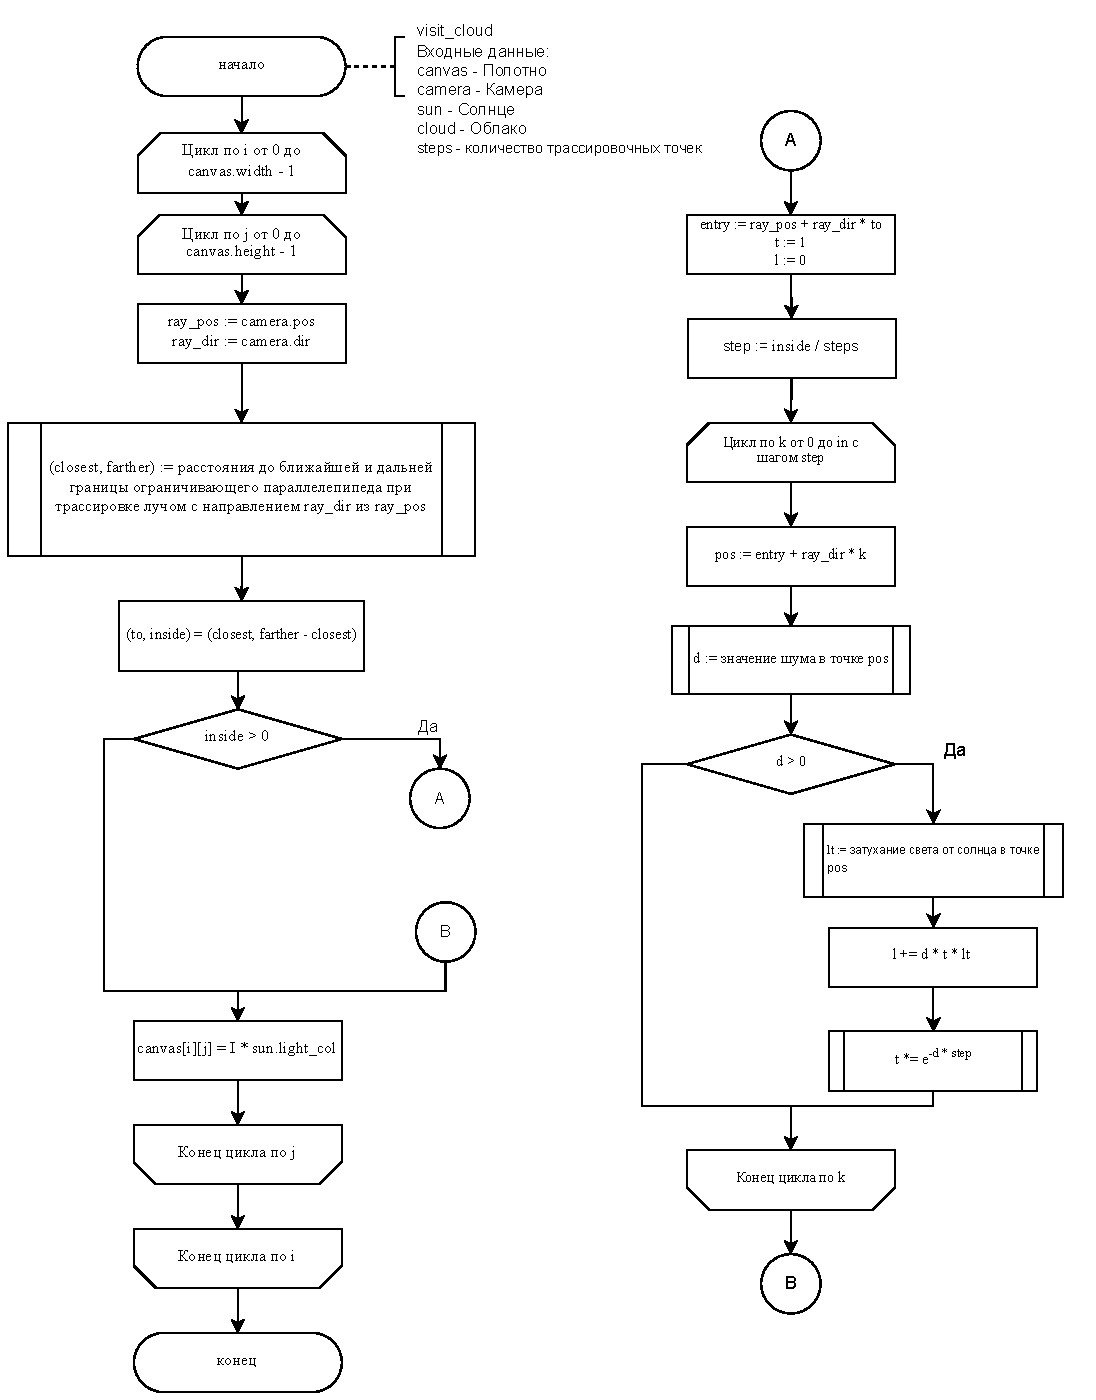
\includegraphics[width=1.05\textwidth, page=1]{assets/img/cloud_flowchart.pdf}   
	\caption{Схема алгоритма отрисовки облака}
	\label{fig:cloud_fc}
\end{figure}

\clearpage
На рисунке~\ref{fig:cloud_fc1} представлена схема алгоритма определения затухания света от солнца в точке облака.
\begin{figure}[ht!]
	\centering
	\includegraphics[width=0.72\textwidth, page=2]{assets/img/cloud_flowchart.pdf}   
	\caption{Схема алгоритма определения затухания света от солнца в точке облака}
	\label{fig:cloud_fc1}
\end{figure}
\clearpage
На рисунке~\ref{fig:cloud_fc2} представлена схема алгоритма генерации ландшафтной сетки из треугольников.
\begin{figure}[ht!]
	\centering
	\includegraphics[width=1.0\textwidth, page=3]{assets/img/cloud_flowchart.pdf}   
	\caption{Схема алгоритма генерации ландшафтной сетки.}
	\label{fig:cloud_fc2}
\end{figure}
\clearpage
На рисунке~\ref{fig:cloud_fc3} представлена схема алгоритма отрисовки ландшафта.
\begin{figure}[ht!]
	\centering
	\includegraphics[width=1.0\textwidth, page=4]{assets/img/cloud_flowchart.pdf}   
	\caption{Схема алгоритма отрисовки ландшафта.}
	\label{fig:cloud_fc3}
\end{figure}
\clearpage
\section{Диаграмма классов}
На рисунке~\ref{fig:uml} представлена UML-диаграмма классов программного обеспечения.

\begin{figure}[ht!]
	\centering
	\includesvg[width=1.0\textwidth]{cloud_uml.svg}   
	\caption{UML-диаграмма}
	\label{fig:uml}
\end{figure}

Операции производятся командами через фасад, который управляет элементами сцены через менеджеров -- это позволит программе не зависеть от интерфейса. 

Менеджер сцены управляет её элементами: облако, ландшафт и солнце.

Менеджер камеры управляет камерой, для которой можно задавать точку наблюдения \textit{pivot} и удаление от неё \textit{distance}, рыскание \textit{yaw} и тангаж \textit{pitch}.

Менеджер отрисовки обращается к менеджерам сцены и камерой и передает камеру и элементы сцены в посетителя--отрисовщика для отрисовки последних.

Облака и ландшафт используют шум Перлина или Ворли---Вороного. Для получения значения шума в определённой точке облака используется метод \textit{sample\_density}. Облако и ландшафт так же хранят ограничивающий параллелепипед, задаваемый двумя точками \textit{min\_max} в пространстве.

\section*{Вывод}
В разделе спроектировано разрабатываемое программное обеспечение и описана декомпозиция разрабатываемого ПО с формальным описанием используемых алгоритмов.
